В настоящата глава се изследват 6 на брой различни разработки за определяне на координатите на получатели на ултразвуков сигнал и за използваните методи и техники. За всеки изследван метод се счита, че позиционирането на получателите е в ъглите на региона, в който се използва системата. Ако региона, в който се използва системата няма ъгли, то тогава получателите се позиционират възможно най-далеч един от друг. 

\subsection{Метод на най-малките квадрати} \label{squares_algorithm}

Изпозлвайки метода на най-малките квадрати представен в \cite{leastsq} се демонстрира намиране на решение чрез разширение на Теоремата на Питагор за 3D. За да се трансформира горната задача в математически модел е нужно да имаме anchor\cite{leastsq2}, което преставлява ориентировъчна точка в пространстовото, в което ще определяме координатитите. За anchor обект избираме позицията на първия получател във виртуалното пространство. Позицията в пространтовото на получателите е константно и е известно винаги.


\begin{equation} \label{pytEq}
   (x-x_i)^2 + (y-y_i)^2 + (z-z_i)^2=d_i^2
\end{equation}

Уравнение \ref{pytEq} описва взаимовръзката между разстоянието и координатите на два обекта. За да генерализираме уравнението, с индекс \textit{l} означаваме стойностите за anchor обекта. Чрез трансформация на уравнението се достига до следния запис:

\begin{equation} \label{pytEqTransformed}
  2 x (x_i - x_l) - 2 y (y_i - y_l) - 2  z  (z_i - z_l) = d^2_i - d^2_l - k_l + k_i
\end{equation}

За краткост в уравнение \ref{pytEqTransformed} променливата \textit{k} е означена като: 
\begin{equation} \label{kdesc}
    k_i= x^2_i + y^2_i + z^2_i
\end{equation}

Следното матрично уравнение служи за намиране на координатите:\\

\centerline{
    $
    2 \begin{bmatrix}
        (x_2-x_1) & (y_2 - y_1) & (z_2 - z_1)\\
        (x_3-x_1) & (y_3 - y_1) & (z_3 - z_1)\\
        (x_4-x_1) & (y_4 - y_1) & (z_4 - z_1)
    \end{bmatrix}
    $
    $
    \begin{bmatrix}
        x\\y\\z
    \end{bmatrix}
    $
    =
    $
    \begin{bmatrix}
        d^2_1 - d^2_2 - k_1 + k_2\\
        d^2_1 - d^2_3 - k_1 + k_3\\
        d^2_1 - d^2_4 - k_1 + k_4\\
    \end{bmatrix}\\
    $
}\\

Уравнението може да бъде решено от множество пакети за компютърна математика включително от MathNet Numerics \cite{numerics}.

\pagebreak

\subsection{Метод за следене използвайки ултразвук за увеличена реалност}

В документ \cite{vr} се описва система изградена от 4 получателя, които са позиционирани в ъглите на региона. Описани са 3 равнини [фиг. \ref{fig:planes}], които се използват за изчислението на координатите на точките. Това е еквивалентно на линеризиране на уравненията, за което в \cite{murphy} е споменато като метод, който не дава задоволителни резултати в реални условия.  Изчисленията на координатите се извършват с помощта на  Питагоровата теорема. За целта се използват  следните уравнения. \\

\centerline{
    \begin{equation}
        k=i+2
    \end{equation}
}

\centerline{
    \begin{equation} \label{22eq}
        \begin{bmatrix}
                $(x_i - x)^2 + y^2 = d_i_2$\\
                $(x_k - x)^2 + y^2 = d^2_k$
        \end{bmatrix}
    \end{equation}
}

\begin{figure}
    \centering
    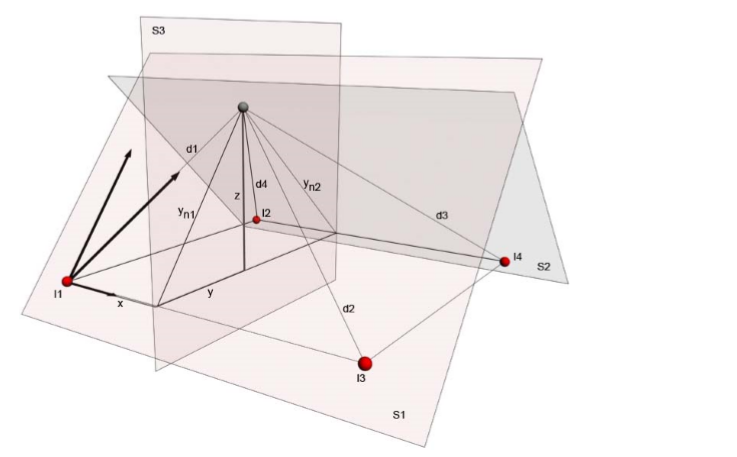
\includegraphics{planes}
    \caption{Равнините използвани за пресмятането на координатите}
    \label{fig:planes}
\end{figure}

\pagebreak

\subsection{Определяне на позиция в 3 измерения с помоща на трилатерация и приблизителни разстояния}

В документ \cite{murphy} е разработена система за следене на товарите в 3 измерения в мина чрез използване на трансмитери и получатели [фиг. \ref{fig:mine}]. Използвани са радио трансмитери. Разработен е специализиран лазер, който изчислява височината на товара, без който проблема за 3 измерения се е считал за нерешим. Проблем представляват разликите във височината и останалите измерения тъй като останалите измерения са в пъти по-големи в повечето случаи, както се вижда във фигура \ref{fig:initPos}, тъй като това тази разлика често води до изродени матрици.

\begin{figure}
    \centering
    \centerline{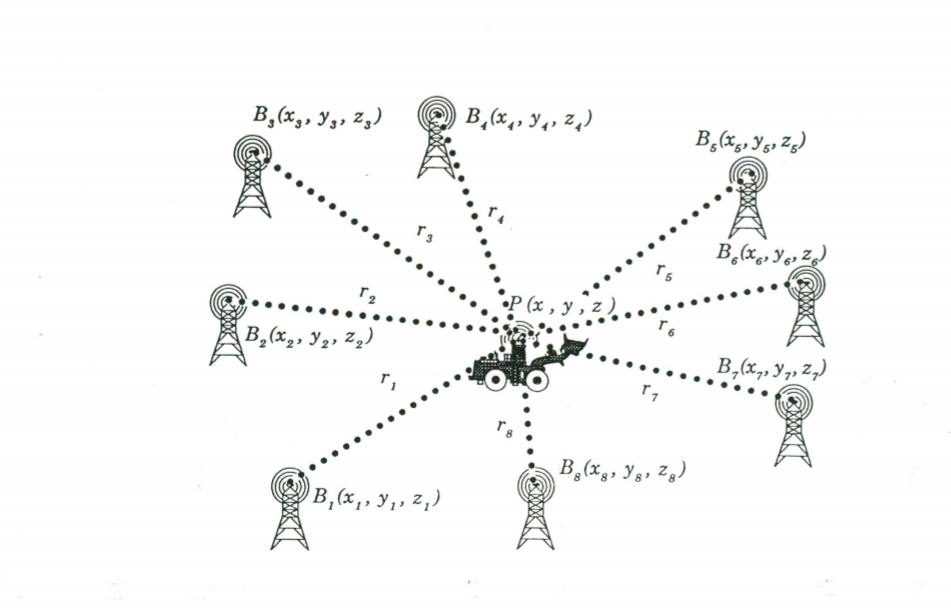
\includegraphics{dt1}}
    \caption{Разположение на получателите и предавателя в мина}
    \label{fig:mine}
\end{figure}

\begin{figure}
    \centering
    \centerline{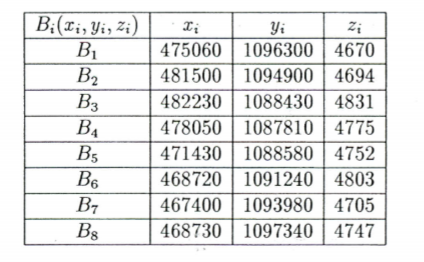
\includegraphics{MurphyInitialPositions}}
    \caption{Начално разположение на статичните получатели}
    \label{fig:initPos}
\end{figure}


\begin{equation}\label{circleEq}
    (x-x_i)^2 + (y-y_i)^2 +(z-z_i)^2=r_i^2
\end{equation}

Разглежда се възможността за съствяне система от \textit{N} на брой нелинейни уравнения използвайки формулата за сфера (уравнение \ref{circleEq}). Задачата се моделира като търсене на пресечни точки на N на брой сфери за всеки трансмитер.

Решението на гореспоменатата нелинейна система от уравнения \emph{се счита за неоптимално} тъй като полученото уравнение е нелинейно и е от висока степен. Когато разстоянията, които са измерени са точни, а не са приблизителни, линезирането на системата от уравнения е удачно. В този случай задачата се преобразува в търсенето на пресечната точка на няколко равнини. Системи с по-малко от тази бройка приемници се считат за неизползваеми. \\

Разглежда се метод за линеризация на уравненията, за който всяка измерена дистанция между трансмитер и получател се използва уравнението за сфера ( кръг в 2D ) ( уравнение \ref{circleEq} ). Методът за линеризация съвпада с този използван в секция \ref{squares_algorithm}. Тъй като има (n-1) уравнения, за долна граница се считат 4 бр. приемника.
\\

Разглеждат се няколко метода за работа с приблизителни разстояния

\begin{itemize}
    \item \strong{Линейни най-малки квадрати} \\ Този метод предоставя по-задоволителни резултати в сравнение с решаване на проблема чрез решение на задачата с линеризиране на уравненията, но не дава оптимални резултати, защото резултатите определят координатите с  грешка повече от 5 фута, което в ситуацията описана в статия \cite{murphy}, е недостатъчно като точност. Тъй като разстоянията са приблизителни се решава уравнение \ref{matrixeq}. Чрез минимизиране на сумата на квадратите на остатъците, уравнение \ref{nonNormalEq} води до уравнение \ref{normalEq}. \textit{[Noble and Daniel 1988]}
    
    \begin{equation} \label{matrixeq}
      A \vec{x} \approx \vec{b} 
    \end{equation}
    
    \begin{equation} \label{nonNormalEq}
        S = \vec{r}^T \vec{r} = (\vec{b} - A \vec{x})^T ( \vec{b} - A \vec{x})
    \end{equation}
    
    \begin{equation} \label{normalEq}
        A^T A \vec{x} = A^T \vec{b}
    \end{equation}
    
        
    Ако матрицата A в изразa $A^T A$ на уравнение \ref{normalEq} не е изродена се използва уравнение \ref{nonSing} , за да се намери решение на задачата.

    \begin{equation} \label{nonSing}
        \vec{x} = (A^T A)^{-1} A^T \vec{b}
    \end{equation}
    
    \item \strong{Нелинейни най-малки квадрати}
    
\end{itemize}


\strong{Резултати}

\begin{figure}
    \centering
    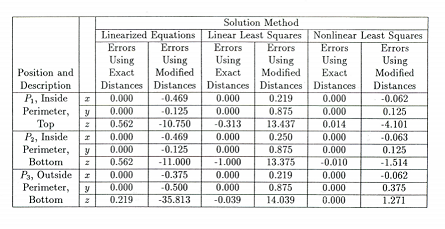
\includegraphics{murphyresults}
    \caption{Резултати при използване на различни методи за изчисление}
    \label{fig:murphyResults}
\end{figure}



Фигура \ref{fig:murphyResults} демонстрира резултатите при определянето на координатите. Най-добри резултати се получават при използването на нелинейни най-малки квадрати, а най-лоши при използването на линеризирани уравнения. Линейните най-малки квадрати водят до най-добри резултати, когато не съществува голяма разлика в стойностите на измеренията (x,y,z).

\pagebreak

\subsection{An Active Tracking System using IEEE 802.15.4-based Ultrasonic Sensor Devices}

В документ \cite{yonei} е имплементирана система за следене на обект в пространството използвайки IEEE 802.15.4 базирани ултразвукови сензори.
IEEE 802.15.4 се използва главно в безжичните сензорни мрежи заради ниската консумация на енергия и бързия обмен на информация между компонентите на системата \ref{fig:yoneiFig}. Системата съдържа 1 движещ се компонент. Координатите на движещия се компонент се изчисляват чрез използване на трилатерация.  Описани са 2 категории системи за обработка и изпращане на ултразвукови сигнали \cite{sysTypes}:

\begin{enumerate}
    \item Активни - движещите компоненти излъчват сигнал, а статичните компоненти получават сигнала и го обработват.
    \item Пасивни - движещите компоненти не излъчват сигнал, а получават сигнал, с който се определя разстоянието до различните получатели.
\end{enumerate}

\begin{figure}
    \centering
    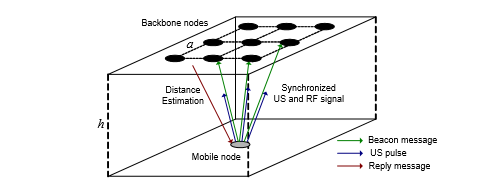
\includegraphics{yonei}
    \caption{Диаграма на разработената система}
    \label{fig:yoneiFig}
\end{figure}


Системата, която е разработена е класифицирана като активна.За коректно пресмятане на координатите на движещия се компонент се изискват измервания от поне 3 бр. статични компонента.



\pagebreak

\subsection{Позициониране чрез независими източници}

В документ \cite{bristolBeacons} се описва пасивна система [фиг. \ref{fig:bristolResults}], в която движещ се обект използва ултразвукови сигнали от няколко източника, за да определи позицията си в пространстовото. Движещия се обект използва разликите в периода на сигнала, което е форма на Доплеров ефект, за да определи своята позиция и скоростта си. Този подход е нов се счита за иновативен в измерването на разстоянието между различните обекти. Различава се от страндартния подход наречен time of flight (TOF), който се използва в текущата дипломна работа за измерване на разстоянията. Използвайки измервания на периода на получаване на сигнали, системата успешно идентифицира източника на даден сигнал. За да се гарантира, че приемника правилно ще идентифицира кой е текущия трансмитер, се използват подбрани периоди така че да не се получават конфликтни идентификации. За всеки трансмитер се изчислява, каква е промяната през изминалия период с помощта на зависимостта, която гласи, че изменението на пулса е пропорционално на разстоянието, което получателя е изминал през дадения период. Тази зависимост се изразява в уравнение \ref{prop}.

\begin{figure}
    \centering
    \centerline{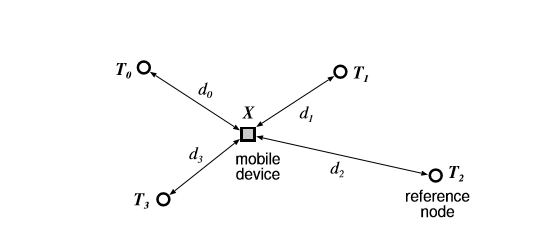
\includegraphics{bristolConfig}}
    \caption{Конфигурация на трансмитери и получатели}
    \label{bristolVis}
\end{figure}


\centerline{\begin{equation} \label{prop}
    \Delta d = v_s \Delta P_i
\end{equation}} \\

Системата се нуждае от поне 7 трансмитера, за да работи. 

За да се определи позицията на обекта се използва Kalman филтър с множество хипотези \cite{kalmanFilter}. За да се определи позицията се ипзолзва формула \ref{kalman}.

\centerline{\begin{equation} \label{kalman}
    ((X-T_i)/ (|X-T_i|)) * V = (\Delta P_i * v_s) / (P_i + \Delta P_i)
\end{equation}}\\

Чрез изпълняванет на много паралелни филтри се генерират хипотези за позицията на обекта в пространстовото. След протичането на този процес хипотезите се комбинират. В документ \cite{bristolBeacons} е решено хипотезите да бъдат комбинирани чрез осредняване на координатите. \\


\strong{Резултати} \\
Чрез използване на Kalman филтър са измерени резултатите изобразени на фиг. \ref{fig:bristolResults}

\begin{figure}
    \centering
    \centerline{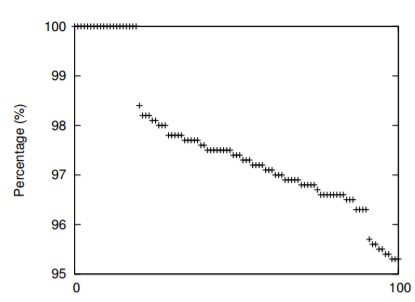
\includegraphics{bristolResults}}
    \caption{Качество на резултатите в проценти, при низходящо сортирани по дистанция данни}
    \label{fig:bristolResults}
\end{figure}

\pagebreak

\subsection{Kalman филтър} \label{kalmanSect}

В документ \cite{kalmanTutorial} се изследва приложимостта на Kalman филтър за определяне на дадена стойност при присъствие на несигурност или неточност в работните данни.

Популярността на Kalman филтър се базира на следните качества, които той притежава

\begin{enumerate}
    \item Добри практически резултати
    \item Удобен е за обработка на данни в реално време
    \item Лесна за реализация имплементация
    \item Измервателните уравнения не трябва да се инвертират
\end{enumerate}

Считайки нормално разпределение на грешката.
\pagebreak

\subsection{Обобщение}


\pagebreak